%페이지 세팅
\documentclass[10pt,a4paper]{article}
\setlength{\parindent}{0em}                  %DISTANCIA SANGRÍA
\setlength{\parskip}{0.5em}                  %DISTANCIA ENTRE PÁRRAFOS
\textwidth 6.5in
\textheight 9.in
\oddsidemargin 0in
\headheight 0in

\usepackage{amsmath}
\usepackage{tcolorbox}
\usepackage{amssymb}
\usepackage{amsthm}
\usepackage{lastpage}
\usepackage{fancyhdr}
\usepackage{accents}
\usepackage{setup}
\usepackage{import}
\usepackage{fancyhdr}
\usepackage{layouts}
\addtolength{\voffset}{0mm}
\addtolength{\textheight}{0mm}

\usepackage{xcolor}
\usepackage{mdframed}
\usepackage[shortlabels]{enumitem}
\usepackage{indentfirst}
\usepackage{hyperref}
    
\renewcommand{\thesubsection}{\thesection.\alph{subsection}}
\linespread{1.15}
% 여기서 변경하는 제목들을 설정해 준다. 
%%
%----------------- 예비레포트 주차 
\newcommand{\numnum}{2}
%-----------------단원명
\newcommand{\subtitle}{wireshark(2) : TCP UDP IP protocols}
%-----------------문제번호들
% \newcommand{\problemnuma}{1}
% \newcommand{\problemnumb}{2}
% \newcommand{\problemnumc}{3}
% \newcommand{\problemnumd}{4}
% \newcommand{\problemnume}{5}
% \newcommand{\problemnumf}{6}
% \newcommand{\problemnumg}{7}
% \newcommand{\problemnumh}{8}
% \newcommand{\problemnumi}{9}
%%%%%%%%%%%%%%%%%%%%%%%%%%%%%%%%%%%%%%%%%%%%%%%%%%%%%%%%%%%%%%%%%%%%%%%%%%
%--> 떠다니는 객체 사용하는 부분 
\usepackage{wrapfig}
\newenvironment{problem}[2][Problem]  
    { \begin{mdframed}[backgroundcolor=gray!20] \textbf{#1 #2} \\}
    {  \end{mdframed}}
%%%%%%%%%%%%%%%%%%%%%%%%%%%%%%%%%%%%%%%%%%%%%%%%%%%%%%%%%%%%%%%%%%%%%%%%%%
\begin{document}
\pagestyle{fancy}
\fancyhf{}
    \rhead{\small 2조 2016142096 조윤신, 2017142043 김재민}
    \lhead{\textsc{Pre Report Week \numnum \quad \subtitle}}
\cfoot{\thepage}
\renewcommand\headrulewidth{0.3mm}
%\renewcommand\footrulewidth{0.3mm}
\thispagestyle{plain}
\begin{flushleft}
\textsc{School of Electrical and Electronic of Enginnering} \\
\textsc{eee 4474-01 : Experiments on Communication Networks }\\[0.1cm]
\small{\textsc{\textbf{2조} 2016142096 \textbf{조윤신}, 2017142043 \textbf{김재민}}}\\
\end{flushleft}

\begin{flushright}\vspace{-25mm}
    
\includegraphics[height=3cm]{image/1.jpg}
    \vspace{5mm}
\end{flushright}
    \begin{center}\vspace{-1.5cm}
        \textbf{\huge  Pre Report Week\numnum}\\ 
        \vspace{0.6mm}
        {\large \subtitle}\\           
    \end{center}
\vspace{-5mm}
\rule{\linewidth}{0.4mm}
\vspace{-5mm}
% main documents
\import{./week02}{01_tcp}
\newpage
\import{./week02}{02_udp}
\newpage
\import{./week02}{03_ip}
\end{document}

% 일반적인 이미지를 사용하는 부분
%%%%%%%%%%%%%%%%%%%%%%%%%%%%%%%%%%%%%%%%%%%%%%%%%%%%%%%%%%%%%%%%%%%%%%%%%%
bla. \\
    \vspace{-4mm}  
        \begin{figure}[!h]\centering
    		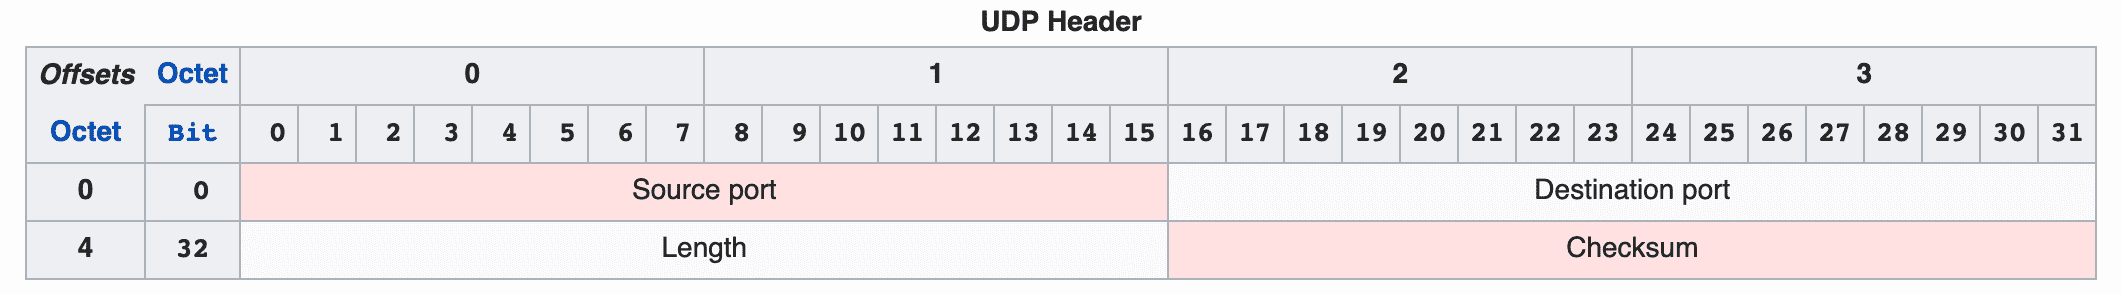
\includegraphics[width=.9\textwidth]{image/week01/2-1.png}
    		\caption{\small UDP Header}
    		\vspace{-10pt}
        \end{figure}
%%%%%%%%%%%%%%%%%%%%%%%%%%%%%%%%%%%%%%%%%%%%%%%%%%%%%%%%%%%%%%%%%%%%%%%%%%
